% \documentclass[fontset=myfounderx, twoside]{ctexart}
\documentclass[twoside]{ctexart}
\usepackage{graphicx}

\ExplSyntaxOn

\usepackage{geometry, multicol, setspace, xeCJKfntef}
\usepackage{mathtools, unicode-math}
% \usepackage{libertinus}
% \setmainfont{Libertinus~Serif}[Ligatures={TeX, Discretionary}]
% \setmonofont{Iosevka~Curly~Slab}

% % ultra-condensed
% \geometry{ a4paper, vmargin=4bp, outer=2bp, nomarginpar, ignoreheadfoot, textwidth=590bp }
% % 590 = (39 * 2) * 7.5 + 5, 39 char per line
% \dim_gset:Nn \columnsep     { 5    bp }

\geometry { a4paper, vmargin=5bp, outer=4bp,
nomarginpar, ignoreheadfoot, textwidth=585bp }
% 585 = 78 * 7.5bp, 38.5 char per line.
\dim_gset:Nn \columnsep     { 7.5  bp }

\dim_gset:Nn \columnseprule { 0.5  bp }
\dim_gset:Nn \fboxsep       { 0.75 bp }
\dim_gset:Nn \fboxrule      { 0.75 bp }

\NewDocumentCommand { \widthonly } { m }
{
  \hbox_set:Nn   \l_tmpa_box { #1  }
  \box_set_ht:Nn \l_tmpa_box { 0bp }
  \box_set_dp:Nn \l_tmpa_box { 0bp }
  \box_use:N     \l_tmpa_box
}

\NewDocumentCommand{ \mybox } { m }
{ \widthonly { \fbox{ #1 } } \c_space_tl }

\NewDocumentCommand{ \myul } { m }
{ \widthonly 
  { \CJKunderline [ thickness=0.75bp, depth=1.5bp ] { #1 } } 
  \c_space_tl }

\ctexset{
  punct=kaiming,
  section = {
    format=\zhbf,
    format+=\mybox,
    runin=true,
    beforeskip=1bp,
    afterskip=0bp,
    aftername=\c_space_tl,
    aftertitle={},
  },
  subsection = {
    format=\zhbf,
    format+=\myul,
    runin=true,
    beforeskip=0bp,
    afterskip=0bp,
    aftername=\c_space_tl,
    aftertitle={},
  },
  subsubsection = {
    format=\bfseries,
    runin=true,
    beforeskip=0bp,
    afterskip=0bp,
    aftername=\c_space_tl,
    aftertitle=\c_space_tl,
  },
}

\ProvideDocumentCommand { \zhbf } {} { \sffamily \heiti }
\NewDocumentCommand { \zhemph } { +m } { { \zhbf #1 } }
\NewDocumentCommand { \zhii }   { +m } { { \zhbf #1 } }

\ExplSyntaxOff

\begin{document}

\pagestyle{empty}
\setstretch{1.1}
\zihao{6}

\begin{multicols}{2}
  \section{分布式系统的定义} 分布式系统是若干独立计算机的集合,这些计算机对于用户来说就像是单个相关的系统。 为了使种类各异的计算机和网络都呈现为单个的系统,分布式系统常常通过一个``软件层''组织起来,该``软件层''在逻辑上位于有用户和应用程序组成的高层与有操作系统组成的低层之间。这样的分布式系统又称为\zhemph{中间件(middleware)}。\zhemph{目标:} \zhemph{使资源可访问、透明性、开放性、可扩展性} 
  
  \zhemph{透明的类型} \textbf{访问透明性、位置透明性、迁移透明性、重定位透明性、复制透明性、并发透明性、故障透明性}
  
  \section{分布式系统的类型} \zhemph{分布式计算系统} 用于高性能计算任务的系统。 (\zhemph{集群计算系统} 底层硬件是由类似的工作站或PC集组成,通过高速的局域网紧密连接起来的。而且,每个节点运行的是相同的操作系统。集群计算系统的特点是同构性,大多数情况下,集群中的计算机都是相同的:有相同的操作系统 通过同一网络连接 \zhemph{网格计算系统}) \zhemph{分布式信息系统} \zhemph{分布式普适系统}

  \zhemph{体系结构的样式} 1.分层体系结构 2.基于对象的体系结构 3.以数据为中心的体系结构 4.基于事件的体系结构 非集中式体系结构 结构化的点对点体系结构 \zhemph{点对点体系结构} 在结构化的点对点体系机构中,覆盖网络是一个确定性的过程来构成的。这个使用最多的进程是通过一个分布式哈希表来组织进程的  \zhemph{非结构化的点对点体系结构} 很多非结构化的点对点系统的一个目标就是构造一个类似于随机图的覆盖网络     
  
  \zhemph{虚拟化的分类} 1.在应用层2.在函数层3.在操作系统层4.硬件抽象层做虚拟化:对各种硬件去做虚拟化5.在指令架构做虚拟化:把一个指令集翻译成另外一个指令集
  
  \zhemph{虚拟机体系结构} 进程虚拟机(process virtual machine) 虚拟机监视器(virtual machine monitor, VMM),例如VMware 
  
  \zhemph{服务器的类型} lterative:一次只能处理一个 Concurrent:同时处理多个请求 
  
  \zhemph{服务器集群} 第一层:利用负载平衡器分发请求 第二层:服务器集群 第三层:与数据打交道

  \section{P2P} \zhemph{广泛部署的P2P系统:}

  \zhemph{Napster}特点: 中心化的P2P系统,拥有集中的服务器用于维护文件索引。工作原理: 用户通过Napster服务器查找其他用户的文件,然后直接连接到这些用户进行文件共享。问题: 面临版权问题,因为Napster服务器集中维护了所有文件的索引,导致法律纠纷最终关闭。
  
  \zhemph{Gnutella}特点: 去中心化的P2P协议,没有中心化的服务器,每个节点充当对等方。工作原理: 用户通过网络直接连接到其他用户,共享文件。每个节点都可以充当客户端和服务器。问题: 可能面临搜索效率和网络流量问题,因为查询需要在整个网络中传播。

  \zhemph{Fasttrack}特点: 混合了中心化和去中心化的结构,采用了超节点的概念。工作原理: 超节点协助进行搜索,但实际文件传输仍然是直接的对等连接。问题: 中心化的超节点可能成为单点故障,同时也可能引入一些安全和隐私问题。

  \zhemph{BitTorrent}特点: 分布式文件共享协议,强调下载者也是上传者,促使用户共享资源。工作原理: 文件被分成小块,下载者从多个源同时下载这些块,提高下载速度。上传者也分享已下载的块。优点: 高效利用带宽,减轻服务器负担,用户共享越多,下载速度越快。

  \zhemph{具有可证明属性的P2P系统:}
  
  \zhemph{Chord}特点: 分布式哈希表协议,旨在提供在大规模P2P网络中快速查找键-值对的能力。工作原理: 使用一致的哈希函数,确保均匀分布数据,并通过指向的方式连接节点,实现对等方之间的快速查找。优势: 具有可证明的性能和一致性属性,适用于大规模网络。

  \zhemph{Pastry}特点: P2P覆盖网络协议,具有自组织和自适应特性。工作原理: 使用哈希表进行消息路由,节点之间通过相邻的哈希值连接,形成自适应的拓扑结构。优势: 高度可扩展,能够适应网络拓扑的变化。

  \zhemph{Kelips}特点: 适用于分布式哈希表的P2P系统,具有高度的可扩展性。工作原理: 采用一种自适应的拓扑结构,将数据存储在多个节点上,以提高容错性和性能。优势: 具有高度的可扩展性和容错性,适用于大规模P2P网络。

  \section{通信} 目前主要有四种方法用于进程间通信 - IPC models: RPC RMI MOM Streams \zhemph{分层协议 - Layered Protocols} 分层协议可以解决通信的问题 \zhemph{两大类协议} 面向连接 消息发送与接收双方需要先建立连接,再传输数据;面向无连接 直接传数据 \zhemph{中间件协议} 中间件是一种应用程序,逻辑上位于应用层中。中间件通信协议支持高层通信服务;对实时数据传输进行设定并使其保持同步的协议;还提供可靠的多播服务。

  \zhemph{远程过程调用 - Remote Procedure Call} RPC就是一个机器调用位于其他机器上的进程。 A机器的进程调用B机器的进程:A将本地调用进程挂起; A通过参数将信息传递给B; B执行被调用进程; B执行结束将信息传回给A。一般说的RPC就是同步RPC,如上面的流程所示,机器A的调用进程:无需保护现场; 在结果返回之前会阻塞的。

  \zhemph{基本的RPC操作 - Basic RPC Operation} RPC操作背后隐含的思想是尽量是\zhemph{远程过程调用具有与本地调用相同的形式}。 将客户过程对客户存根发出的本地调用转换成对服务器过程的本地调用,而客户和服务器都不会意识到有中间步骤的存在 使用socket进行通信,把socket通信隐藏到底层,从而实现透明性。

  \zhemph{RPC的步骤}:\zhemph{总结一下就是}:发送:客户过程 $\to$ 客户存根 $\to$ 客户操作系统 $\to$ 服务器操作系统 $\to$ 服务器存根 $\to$ 服务器进程 返回:从右向左就是了 \zhemph{具体}:客户过程以正常的方式调用客户存根;客户存根生成一个消息,然后调用本地操作系统;客户端操作系统将消息发送给远程操作系统;远程操作系统将消息交给服务器存根;服务器存根将参数提取出来,然后调用服务器;服务器执行要求的操作,操作完成后将结果返回给服务器存根;服务器存根将结果打包成一个消息,然后调用本地操作系统;服务器操作系统将含有结果的消息发送回客户端操作系统;客户端操作系统将消息交给客户存根;客户存根将结果从消息中提取出来,返回给调用他的客户过程。\zhemph{参数传递 - Parameter Passing} 完整定义了RPC协议后,需要实现客户存根和服务器存根,不同点仅仅在于面向应用程序的接口。 接口通常使用\zhemph{IDL}(接口定义语言),用IDL说明的接口可以与适当的编译时接口或者运行时接口一起编译到客户存根过程和服务器存根中。

  \zhemph{异步RPC - Variations} \zhemph{异步RPC中:} 客户发出RPC请求,接受到服务器的确认信息后,不会阻塞,继续向下执行; 服务器在接受到RPC请求后立即向客户送回应答,之后再调用客户请求的过程。异步RPC效率高,但是难编程。

  \zhemph{延迟的同步RPC}:就是两个异步RPC结合起来。远程服务器在处理请求时,客户同时做一些其他的事情。当服务器处理好请求时,返回结果去中断客户,服务器一端变成发送端,实现第二个异步RPC。

  \zhemph{面向消息的通信 - Message-oriented Communication} \zhemph{套接字} 一种通信端点。如果应用程序要通过底层网络发送某些数据,可以把这些数据写入套接字,然后从套接字读出数据。服务器一般执行前4个原语,一般按照图中顺序执行。调用套接字原语的时候,调用者创建一个新的通信端点,用于某种特定的传输协议的。 \zhemph{消息传递接口 MPI} \zhemph{MPI}的先进之处:程序的硬件独立性需要导致MPI的出台。MPI是为并行应用程序设计的,是为瞬时通信量身定做的。它直接使用的是底层网络。MPI是并行计算,一般运行于集群中 \zhemph{消息队列系统} 面向消息的中间件服务。为持久异步通信提供多种支持。\zhemph{本质}是,提供消息的中介存储能力,这样就不需要消息发送方和接收方在消息传输中都保持激活状态。与套接字和MPI的重要\zhemph{区别}在于,它的设计目标一般是支持那些时间要求较为宽松的消息传输,不适合几秒甚至几微秒内要完成的传输。

  \zhemph{面向流的通信 - Stream-oriented Communication} \zhemph{简单流}:只包含单个数据序列;\zhemph{复杂流}:简单流的组合 \zhemph{传输模式} 1.\zhemph{异步传输模式}:流中的数据项是逐个传输的,但是对某一项在何时进行传输并没有进一步的限制。这是采用离散数据流时常见的情况。比如文件的传输。2.\zhemph{同步传输模式}:数据流中每一个单元都定义了一个端到端的最大延迟时间,容许延迟。数据单元的传输时间是否远远小于最大允许延迟并不重要。3.\zhemph{等时传输模式}:数据单元必须按时传输,端到端的延迟时间同时又上限和下限。这个上、下限也称为边界延迟抖动。在视频和音频方面很常用,比如音视频的同步(对口型)。流媒体就属于这个类,既有最大端到端延迟限制,又有最小的端到端延迟限制。

  \zhemph{流与服务质量} \zhemph{QoS服务质量:} 数据传输所要求的比特率; 创建会话的最大延时(比如应用程序何时可以开始发送数据); 端到端的最大延时; 最大延时抖动; 最大往返延时 \zhemph{QoS保证:}使用 buffer 来减少 jitter.当数据包有不同的延时,接收方先把它们存储在缓冲区,当总是有足够的数据包进入缓冲区时,接收方就可以以固定的速率把数据包传递给应用程序; 针对丢包情况,interleaving,若没有交错机制,丢包时会把连续的几帧一起丢掉,视觉影响较大;而使用交错机制,会交叉丢包。如在传送音视频时,采用交错传输,丢失的帧分布较广,这样丢失的就不是一大段而是零散的帧,对于音视频的播放影响就较小。但是这样需要更大的缓冲区,因此程序的开始延时更高。

  \zhemph{流同步} \zhemph{音视频流同步} 采用音视频的编解码协议:\zhemph{H264协议}

  \section{命名系统 -- Naming} 命名是在分布式中表示这个实体,且要访问到这个实体。访问点:用来实体的一种特殊实体。地址:访问点的名称。所以\zhemph{访问点}就是实体的\zhemph{地址}。

  \zhemph{DHT} 全称是Distributed Hash Tables,是P2P环境下最经典的解决方案 \zhemph{Chord} 使用一个m位的标识符空间,把\zhemph{随机选择}的标识符赋给结点,并把键值赋值给特定实体(任意的东西,比如文件、进程)

  \zhemph{构造Finger table算法:}每个Chord结点维护一个最多有m个实体的指状表(Finger table),如果用\(FT_{p}\)表示结点\(p\)的指状表,那么有:\(FT_{p}\lbrack i\rbrack = succ\left( p + 2^{i - 1} \right)\) 是当前结点; i是指状表的index; \(succ(k)\)表示\(k\)(若结点k存在)或k的下一个\zhemph{存在}的结点,即\(succ(k) \geq k\) \zhemph{解析算法:}目标:从节点p开始解析key=k的结点; 搜索节点p的Finger table,从上依次向下搜索,如果一个结点q满足:\(q = FT_{p}\lbrack j\rbrack \leq k < FT_{P}\lbrack j + 1\rbrack\),那么就将该请求转发给结点q;如果p的Finger table第一个结点就比k还大,即:\(p < k < FT_{P}\lbrack 1\rbrack\), 那么就转发给\(FT_{P}\lbrack 1\rbrack\)结点,此节点负责结点k,将k的地址返回给结点p。

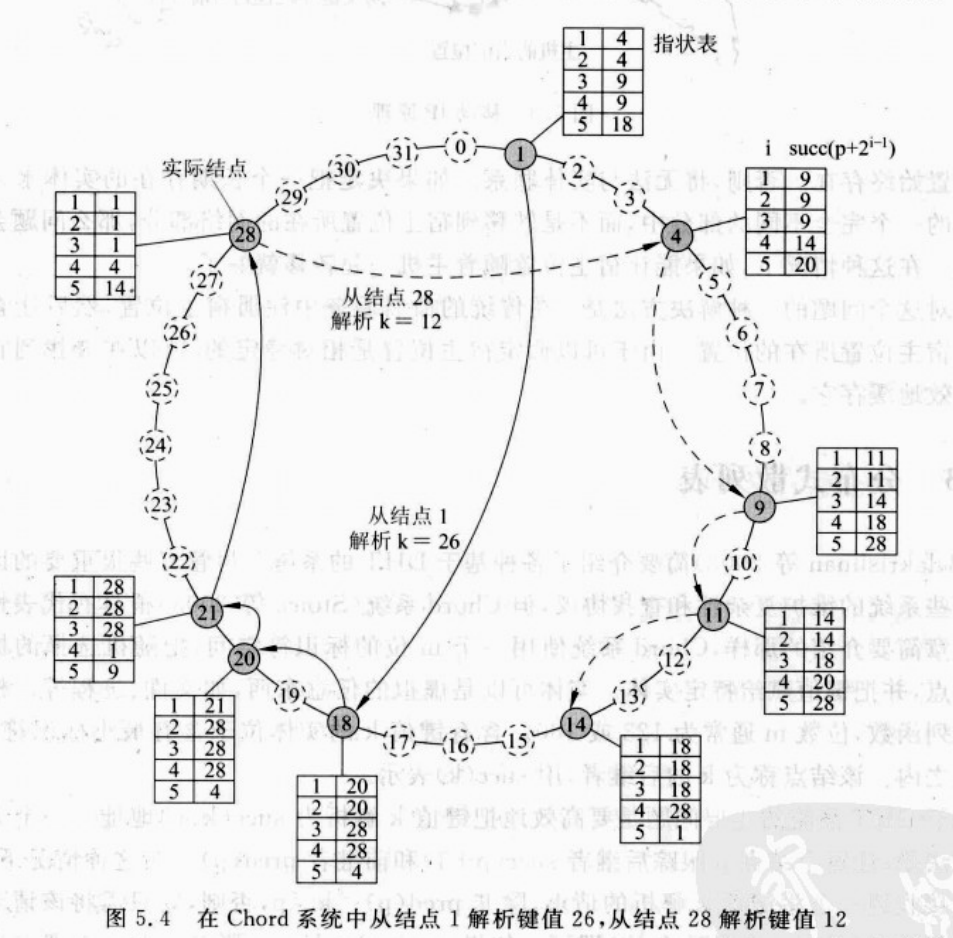
\includegraphics[width=0.45\textwidth,keepaspectratio]{pics/DHT.png}
  
  \zhemph{HLS} 网络被划分为一组域。每个域D都有关联的目录节点dir(D),dir(D)会跟踪域中的实体,形成一颗目录结点树。\zhemph{HLS结构} 为了跟踪实体E的位置,实体E位于域S中,所以域S的目录结点N含有E在该域中的位置信息。而在比域S更高一级的域T中,域T的目录结点N'也有实体E的位置信息,但是这个位置信息只有N的指针,也就是要找实体E,就先去找到其子域的目录结点N,然后通过目录节点N找到E。同理,在比域T更大的域中,那个域的目录节点也有实体E的位置信息,不过这个位置信息只有N'的指针,要找实体E,就要先找N',然后找到N,最后找到E。所以顶级域的目录结点,即根(目录)节点,包括全部实体位置信息。\zhemph{如果一个实体有多个地址} 实体可以拥有多个地址,比如被复制了,实体在域D1和域D2中都有地址,那么同时包含D1和D2的最小域目录结点将有两个指针,每个指针都指向一个包含地址的子域。 \zhemph{HLS查询操作}现在希望能定位实体E的位置信息,那么就向当前域的目录结点发送查找请求,否则向上递归寻找。最差情况是一直找不到,向上转发直到根节点 \zhemph{插入操作} 如果要插入实体E,将其所在域的目录节点加入实体E的地址,然后一路向上转发。如果这个目录结点不知道E,就存储一下子域地址,直到一个节点知道E的位置或者到根节点就终止。\emph{为啥刚刚插入的实体E,可能有的结点已经知道E的位置了呢?}因为E可能是复制过来的,正如上面讲的有多个实体,包含两个E的最小域的目录节点会有E的两个地址,而再往上一层,就只有E的一个地址了(指向两个E的最小域的目录节点),到这里就停止向上传递。 \zhemph{HLS思想} 若用root node实现扁平化直接管理,根节点负载过大,且一旦崩溃,整个集群系统瘫痪。因此,使用分治思想,不同dom内实现自治。

  \zhemph{名称空间的实现} 将名称解析过程以及名称空间管理分布到多台计算机上,通过分布式节点来管理命名图

  \zhemph{全局级别(Global Level):}由高级目录节点组成。其主要特点是这些目录节点必须由不同的管理部门共同管理。\zhemph{管理级别(Administrational Level):}包含可以按照一种方式分组的中级目录节点,以便每个组可以分配给单独的管理部门。\zhemph{管理层级(Managerial Level):}包括单个管理部门内的低级目录节点。主要问题是有效地将目录节点映射到本地名称服务器。

  Global层几乎不怎么变化,Administrational层变化多些,Managerial层变化最多。

  \zhemph{名称解析 - Name Resolution} \zhemph{迭代名称解析 - Iterative Name Resolution 1.}解析请求 \texttt{resolve(dir,{[}name1,…,nameK{]})} 被发送到负责目录 \texttt{dir} 的 \texttt{Server0}。 2. \texttt{Server0} 解析 \texttt{resolve(dir,name1)},得到结果 \texttt{dir1},并返回存储 \texttt{dir1} 的 \texttt{Server1} 的标识(地址)。 3.客户端发送解析请求 \texttt{resolve(dir1,{[}name2,…,nameK{]})} 到 \texttt{Server1},依此类推

  \zhemph{Scalability Issues} \zhemph{Issue 1}: 因为名称解析都需要先解析高级域名,所以高层服务器的需要每秒处理大量处理请求。 \zhemph{Solution:} 因为在global层和administrational层的结点内容几乎不会变,所有我们可以把这些服务器的内容广泛地复制到多个服务器中,这样名称解析可以就近处理,加快速度,如果找不到再发请求到高层服务器。\zhemph{Issue 2}:Geographical scalability - 地域可扩展性,即名称解析服务要可以在很大的地理距离内进行扩展。如果客户和服务器端离的比较远,那么最好采用递归名称解析,因为客户端只和服务器通信一次即可取得结果,而迭代名称解析需要通信多次。

  \section{同步化 -- Synchronization} \zhemph{时钟同步 - Clock Synchronization} \zhemph{Berkeley算法} Berkeley UNIX系统的时间服务器(实际上是时间守护程序)是主动的,定期询问每台机器的时间。然后算出一个平均时间,并告诉所有其他机器将它们的时钟拨快/拨慢一个新的时间。Berkeley算法除了第一次传播时间守护程序的广播外,传播的都是\zhemph{相对时间},如下图的b和c,目的是为了\zhemph{减小误差}。 

  \zhemph{网络时间协议 - network time protocol, NTP} 时间偏差 $ θ=\frac{((T_2-T_1 )-(T_4-T_3))}{2} $ 平均收发延时 $ δ=\frac{((T_2-T_1 )+(T_4-T_3))}{2} $ 取最小的$δ$对应的$θ$值即为最可靠的偏差。根据该偏差即可调整时钟。
  
  \zhemph{逻辑时钟 - Logical clocks} \zhemph{Lamport逻辑时钟} 先发生关系 - Happen-Before (HB) Relation 表达式:a→b读作``a在b之前发生'',意思是所有进程一直认为事件a先发生,然后事件b才发生 HB关系准则: 1.如果a和b是同一进程中的两个事件,且a在b之前发生,则a\emph{→}b为真 2.如果a是一个进程中\zhemph{发送}消息的事件,b是另一个进程中\zhemph{接受}这个消息的事件,那么a\emph{→}b为真 3.如果a→b,b→c,那么a→c

  如何使用HB Relation来维持系统时间一致? 对于每个事件a,我们都能为它分配一个所有进程都认可的时间值C(a) 1.如果a比b先,那么应该是C(a)\textless C(b). 2.若a是发送的,b是接受的,那么应该是C(a)\textless C(b). 若上述两条最后出现了C(a)≥C(b),那么执行操作C(b)=C(a)+1,使得C(a)\textless C(b) \zhemph{注意:调整时钟操作发生在中间件层。} 

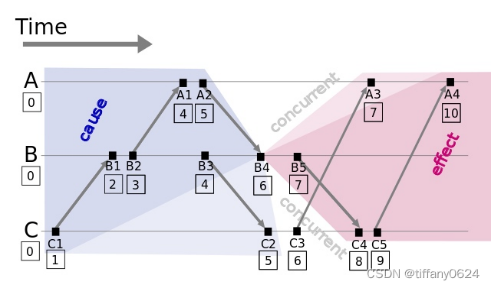
\includegraphics[width=0.45\textwidth,keepaspectratio]{pics/lamport.png}

  \zhemph{全序多播} \zhemph{所谓的全序,就是所有进程统一顺序},只要最后所有进程的事件执行顺序相同就行。进程先给消息打上一个当前逻辑时间作为时间戳,然后把这个消息放进自己的本地队列中,再将这个消息发送给其他进程;进程收到来自其他进程的消息后,也把这个消息放进本地队列中,按时间戳排序。

  \zhemph{向量时钟} 向量时钟可以捕获\zhemph{因果关系} 每个进程都维护一个向量\(VC\),比如进程\(P_{i}\)维护的向量就是\(VC_{i}\),有两个性质: \(VC_{i}\lbrack i\rbrack\)表示目前为止,本进程\(P_{i}\)发生了多少事件;\(VC_{i}\lbrack j\rbrack = k\)表示进程\(P_{i}\)知道\(P_{j}\)已经发生了\(k\)个事件。 执行步骤:\(P_{i}\)进程执行一个事件之前,先把自身的向量里第\(i\)个分量(也就是\(VC_{i}\lbrack i\rbrack\))自增1; \(P_{i}\)进程发送一个消息m给\(P_{j}\)时,把m的时间戳ts(m)设置为等于\(VC_{i}\) ; 接受消息m时,进程\(P_{j}\)通过为每个k设置\(VC_{j}\lbrack k\rbrack = max\left( VC_{j}\lbrack k\rbrack,ts(m)\lbrack k\rbrack \right)\)来调整自己的向量。然后,\(P_{j}\)要执行这个事件,如步骤1所示,把\(VC_{j}\lbrack i\rbrack\)自增1. 

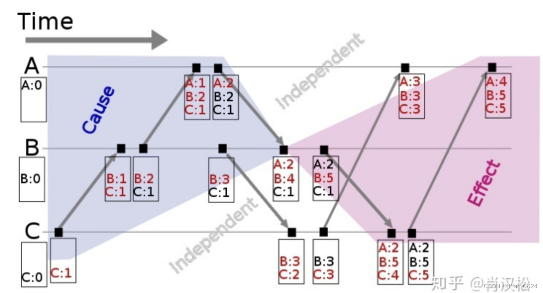
\includegraphics[width=0.45\textwidth,keepaspectratio]{pics/vector.png}

  \zhemph{因果有序多播 causally-ordered multicasting} \zhemph{设计思想:}我懂的不能比你少,不然万一有其他消息还没来,你的消息就插队了,所以我不能收你的消息。 \zhemph{具体操作:} 进程\(P_{i}\)发给进程\(P_{j}\)一个时间戳为ts(m)的消息m。如果不满足以下两个条件,这个消息就不交付给应用层,直到满足条件为止:\(ts(m)\lbrack i\rbrack = VC_{j\lbrack i\rbrack} + 1,\backslash ts(m)\lbrack k\rbrack \leq VC_{j\lbrack k\rbrack},for\ all\ k! = \ i\ \) 关于你刚刚发的消息,可以比我多知道一条消息。毕竟他发的,肯定比我多了解一条;但是关于其他消息,你知道的不可以比我多,不然我就是还有其他消息没收到,等我收到其他消息后再处理这个消息。

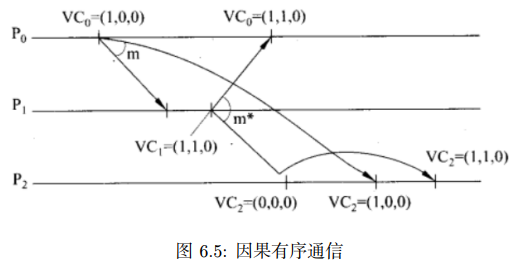
\includegraphics[width=0.35\textwidth,keepaspectratio]{pics/causally-ordered-multicasting.png}

  \zhemph{互斥 - Mutual Exclusion} 分布式系统情况下,进程将需要同时访问相同的资源,互斥算法就是保证进程之间能够互斥访问资源。\zhemph{集中式算法} 选举一个进程作为协调者。其他进程想访问资源都要问他。进程3是协调者,进程1想访问资源,问一下进程3,进程3说ok。进程2也想访问资源,进程3不理进程2,但是把进程2放到等待队列里。进程1用完资源后,向进程3说一声他用完了。进程3便向等待队列的队首进程说一声,可以用资源了。\zhemph{分布式算法} 当一个进程想要某个资源,就向所有其他进程发送消息询问。比如进程A想要一个资源,就向其他进程发消息询问,进程B就收到了A的消息。 若B不想用这个资源,就给A回一个OK.若B已经在用这个资源了,就不理A,但是把A的请求消息放进等待队列中.若B也想用这个资源,但是还没开始用,那么就把A发送来的消息时间戳和自己将要广播消息的时间戳进行比较,谁发的早谁获得资源。\zhemph{这里的一致性是由Lamport逻辑时钟保证的。}竞争失败的进程会给获得资源的进程发个OK,然后把自己放进等待队列里。\zhemph{令牌环算法 - A Token Ring Algorithm} 在网络中,环的顺序是无序的,但是可以用软件的方法构造成一个有序的逻辑环。环的顺序和进程在总线上的位置是无关的。令牌(token)在进程间相互传递,拥有令牌的进程可以访问共享资源,用完就向下传。如果某个进程收到了令牌但不用访问资源就传下去.\zhemph{不允许某一个进程用完资源后,使用同一令牌继续访问该资源}。\zhemph{整个分布式系统中只有一个令牌},如果令牌毁了,比如拥有令牌的进程挂掉了,那么就需要重启一个复杂的分布式进程创建新令牌。

  \zhemph{四种算法的比较} 
  
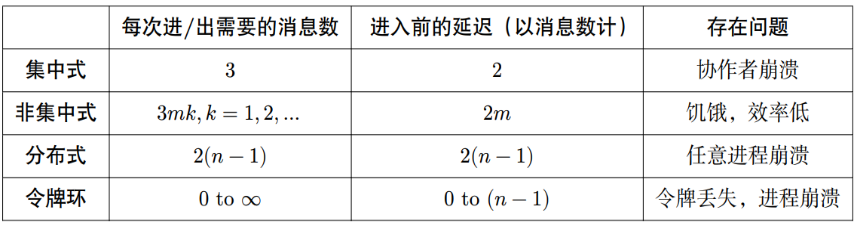
\includegraphics[width=0.35\textwidth,keepaspectratio]{pics/mutex_table.png}

  \zhemph{选举算法 - Election Algorithms} 很多分布式的机子,要选举出一个协调者。或者协调者崩了,要重选一个协调者。\zhemph{选举算法就是选一个协调者的算法,标准:进程ID最大} 
  
  \zhemph{欺负算法 - bully algorithm}  \zhemph{当任何一个进程发现协调者不再响应请求或一个以前崩溃的进程恢复时,发起一次选举}   1.P向所有编号比它大的进程发送一个ELECTION消息  2.如果无人响应,P获胜并称为协调者  如果有编号比它大的进程响应,则由响应者接管选举工作。P的工作完成。

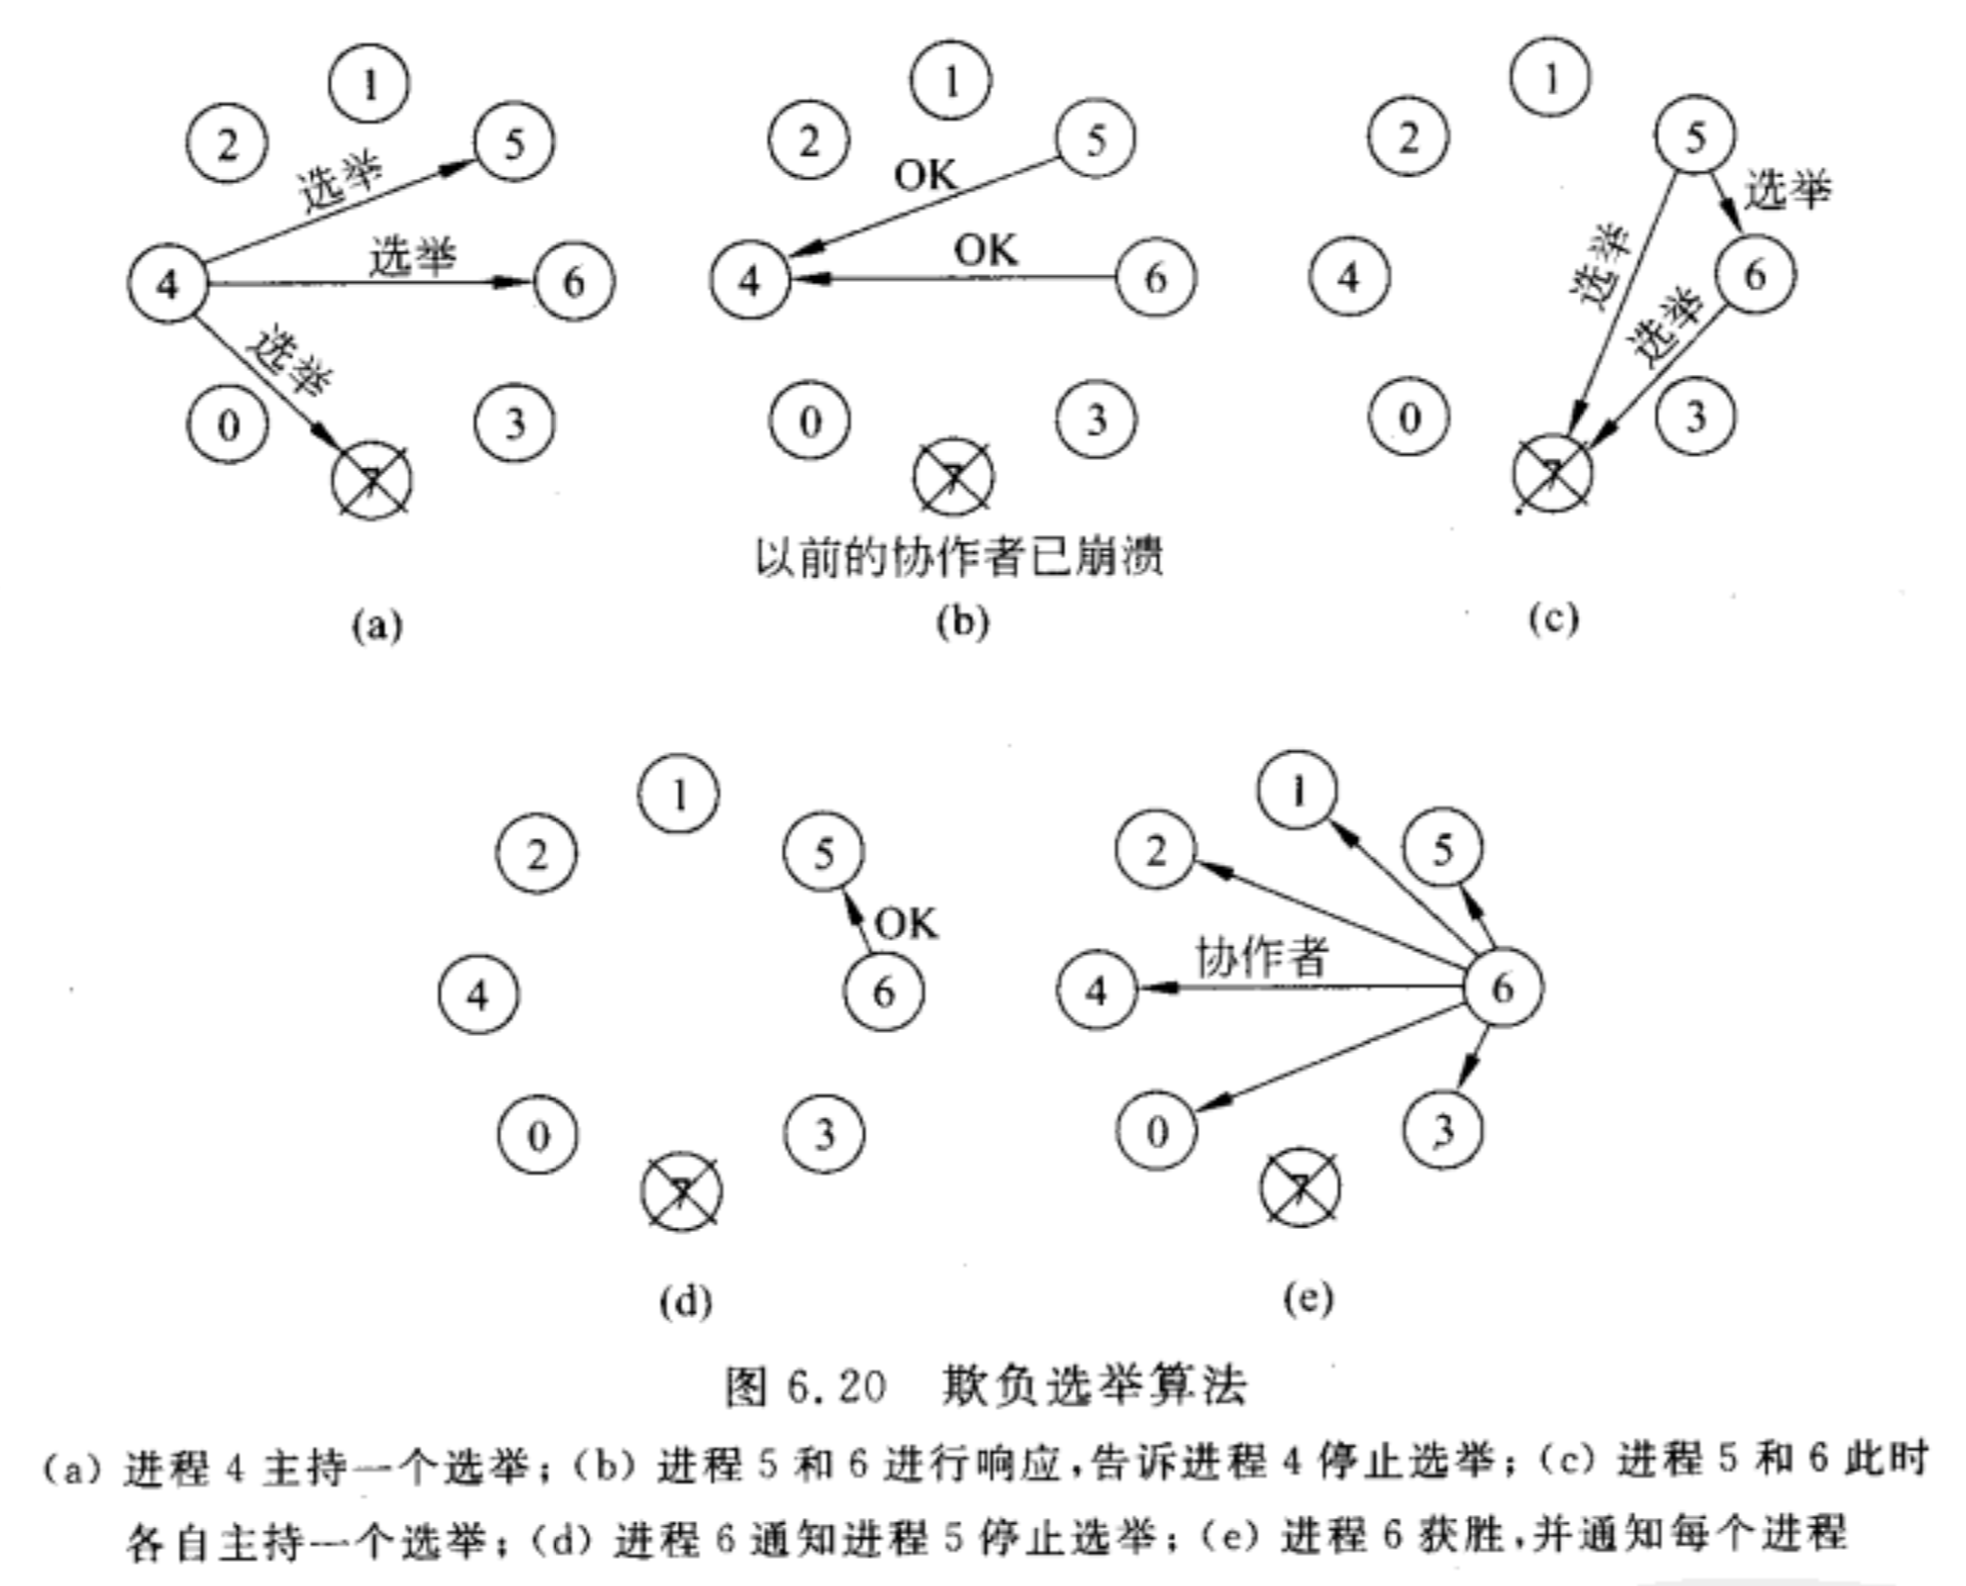
\includegraphics[width=0.45\textwidth,keepaspectratio]{pics/bully.png}

  \zhemph{环算法 - Election in a Ring} 会有2个消息,各绕环一圈。step 1 发送ELECTION message:当任何一个进程发现协调者不工作时,它就构造一个带有它自己进程号的ELECTION消息,发送给后继者。如果后继者崩溃,就跳过崩溃的进程,继续往下走,直到找到一个正在运行的进程。每一步,发送者都将自己的进程号加入到消息中,使自己也成为协调者的候选人。最终消息返回到发起选举的进程。当发起者接收到包含自己号的消息,识别出这个事件,选出进程号最大的作为协调者。step 2 发送COORDINATOR message:第一则的消息转变为COORDINATOR,并再一次绕环运行,通知大家谁是新的协调者以及新环中的成员。消息循环一周后被删除,然后每个进程恢复正常工作

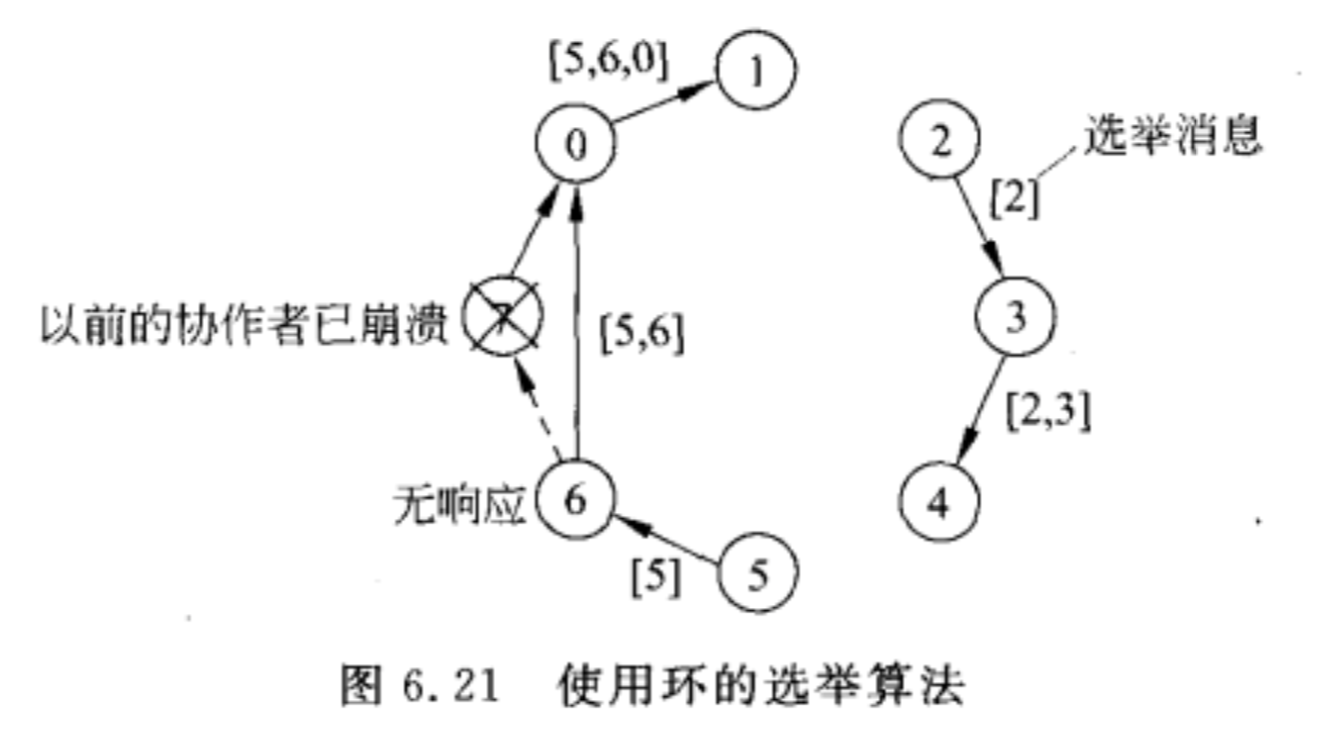
\includegraphics[width=0.35\textwidth,keepaspectratio]{pics/ring.png}

  \section{一致性和复制 - Consistency \& Replication} \zhemph{为什么要进行数据的复制?}进行复制是为了增强系统的\zhemph{可靠性}和\zhemph{性能}。可靠性:更好的防止数据被破坏。性能:当分布式系统需要在服务器数量和地理区域上进行扩展时,就需要复制来提高性能。\zhemph{复制带来的问题 ?}一致性问题 \zhemph{两个术语}\(W_{i}(x)a\)\zhemph{和}\(R_{i}(x)b\) \(W_{i}(x)a\): 进程\(P_{i}\)把数值a写入到数据项x。\(R_{i}(x)b\): 进程Pi从数据项x读取数据后返回数值b。 \zhemph{严格一致性} \zhemph{就是写操作必须在读操作的前面执行} \zhemph{定义:}在一个副本上执行更新操作时,无论这一操作是在哪个副本上启动或执行的,这一更新操作都应该在后序操作发生前传播到所有副本。从这个定义里可以发现:隐含的假设存在绝对的全局时间; 在单处理器中(或者在有单一控制总线环境下-\textgreater 单一时钟)可以实现,在分布式系统中\zhemph{不可能}实现。

  \zhemph{以数据为中心的一致性模型} 不区分客户,所以叫以数据为中心的一致性模型。1.\zhemph{针对所有的用户,是没有区别的。所有用户看到的都是同样的东西。对所有的用户一视同仁。} 2.以数据为中心的一致性模型,从大的范围来看,\zhemph{都是比较严格的一致性模型。 3.成本比较高}。 4.常常用在大型的数据中心中,系统一般来讲不是很大,以局域网为主。 

  \zhemph{以用户为中心的一致性模型} 1.\zhemph{用户不同,看到的结果可能不一样。} 2.以客户为中心的一致性模型,\zhemph{都是比较弱的一致性。} 因为是针对某一个客户的需求来保持一致。3.\zhemph{相对来说成本比较低。} 4.范围广,甚至可以在Internet上使用,相对来说是在一个广域网上,\zhemph{一般用在企业应用上。} 
  
  \zhemph{顺序一致性} \zhemph{定义} 数据存储满足以下条件时,称为是顺序一致的。 任何进程的执行结果都是相同的,就好像所有进程对数据存储的读、写操作是\zhemph{按某种序列顺序}执行的,并且每个进程的操作按照程序所制定的顺序出现在这个序列中。 \zhemph{和严格一致不同之处} 不再要求写必须在读的前面。 \zhemph{思想} 允许由于种种因素出错,但是出的错得是一样的,所有人最后结果相同就行。 

  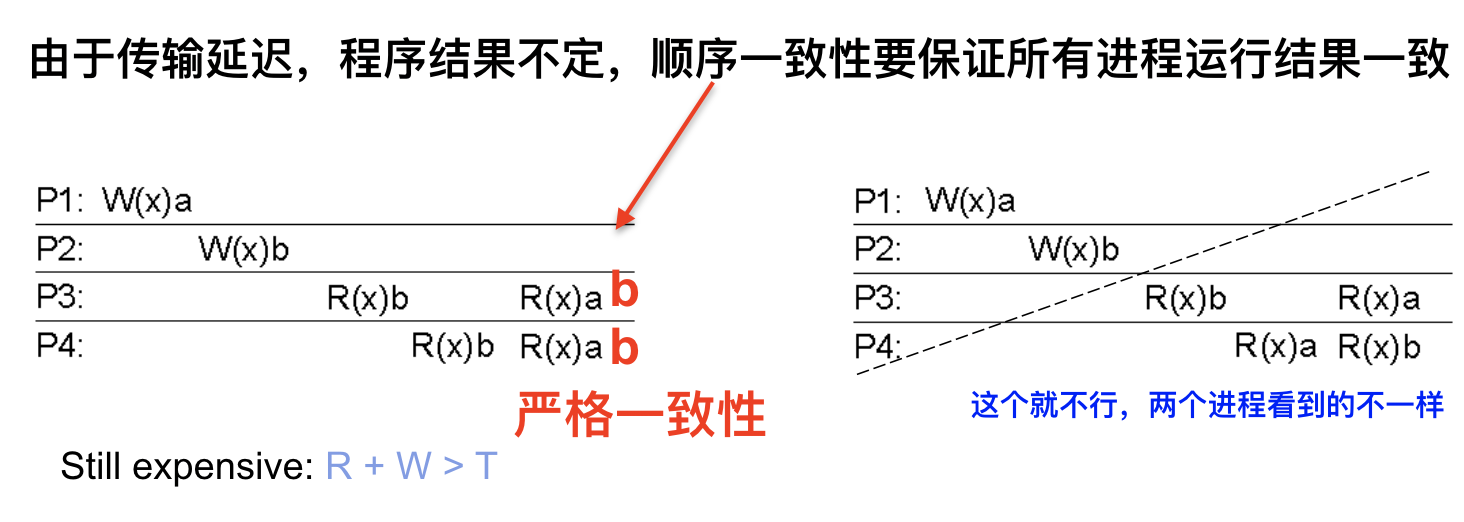
\includegraphics[width=0.45\textwidth,keepaspectratio]{pics/consistency_example1.png}

    不满足顺序一致性:P1和P2不可能都读到0,即使两次write操作是并发的。
    
    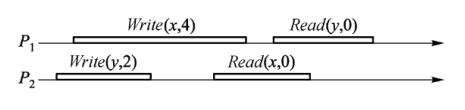
\includegraphics[width=0.25\textwidth,keepaspectratio]{pics/sequential.png}
    
  \zhemph{因果一致性} \zhemph{基本思想} 满足因果条件下,所有人必须是一致的,不满足因果条件可以不一致。从数据的产生和消费的角度去定义因果。数据总是产生在前,消费在后。 \zhemph{因果性} 如果事件B是由事件A引起的,或受到事件A的影响,那么因果关系必然要求其他每个人先看到事件A再看到事件B。考虑一个分布式数据库的示例:假设进程P1对数据项x执行了写操作。然后进程P2先读取x,然后对y执行写操作。这里,对x的读操作和对y的写操作具有潜在的因果关系,因为y的计算可能依赖于P2所读取的x的值(也即,P1写入的值)。 \zhemph{潜在因果关系} 1.\zhemph{同一进程,先读再写有因果关系。}很可能是读取了这个数据才能执行操作,然后写入结果。 2. \zhemph{不同进程,先写再读有因果关系。}不同的进程间,一个把结果写进去,另一个才能够读出来。 3.两个读之间没有因果关系。 4.两个写之间没有因果关系。 5.因果关系具有传递性,e.g. If write1$\to$ read, and read $\to$ write2, then write1 $\to$ write2. \zhemph{定义} 如果数据库是因果一致的,那么它必须服从以下条件:所有进程必须以相同的顺序看到具有\zhemph{潜在因果关系}的写操作。 不同进程上可以以不同的顺序看到并发的写操作。

  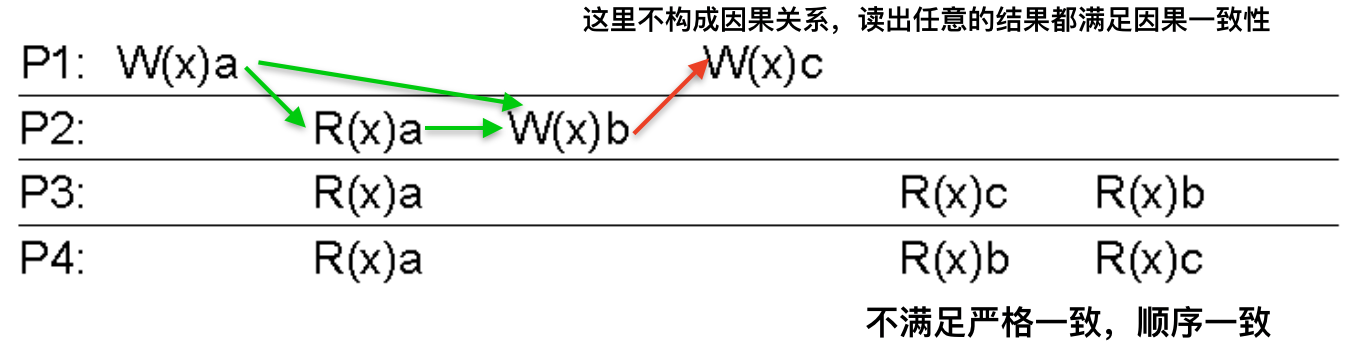
\includegraphics[width=0.35\textwidth,keepaspectratio]{pics/consistency_example2.png}
  
  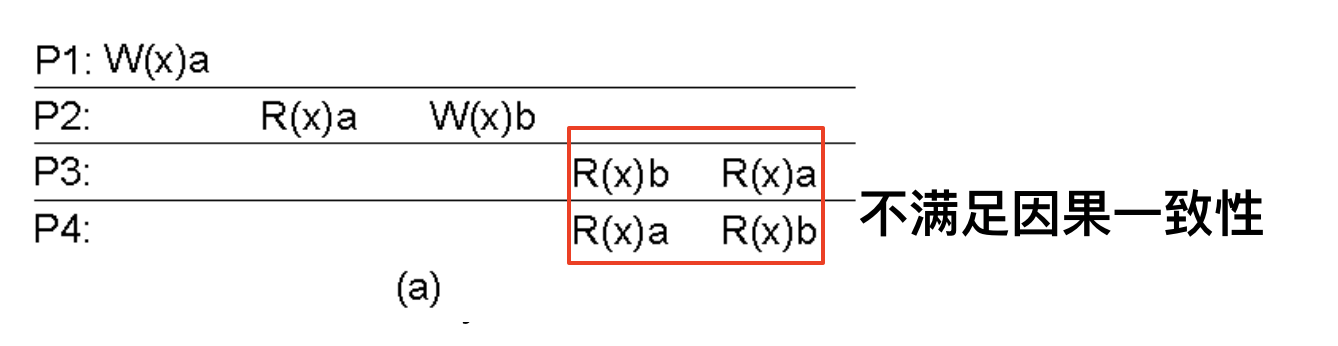
\includegraphics[width=0.35\textwidth,keepaspectratio]{pics/consistency_example3.png}
  
  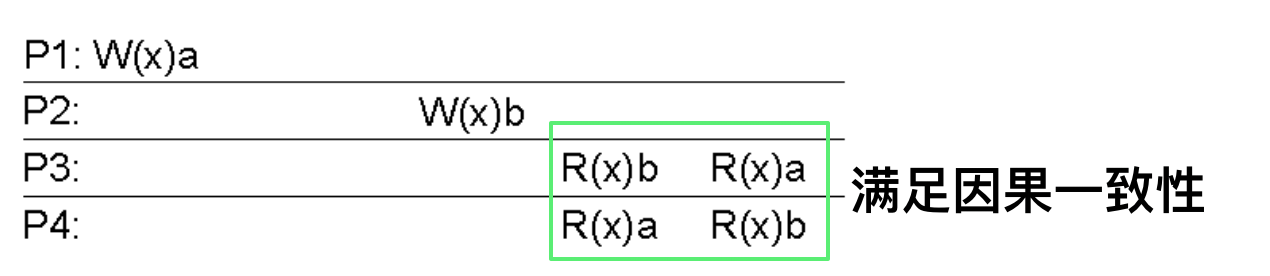
\includegraphics[width=0.35\textwidth,keepaspectratio]{pics/consistency_example4.png}

    不满足因果一致性:那么任何读到了x = 4 的操作就都读不到 x = 2,读到 y = 7 就读不到 y = 4。
    
    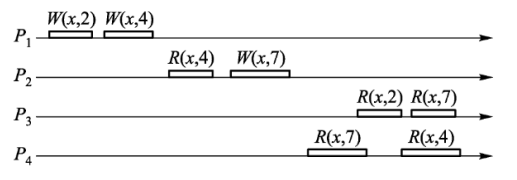
\includegraphics[width=0.25\textwidth,keepaspectratio]{pics/causal.png}
    
  \zhemph{以客户为中心的一致性模型} 底层上是\zhemph{更新的传播}。 \zhemph{最终一致性/事件一致性} 没有更新操作时,所有副本逐渐成为相互完全相同的副本。\zhemph{最终一致性实际上只要求更新操作被保证传播到所有副本。} 常用在广域网,分布式数据库上。
  
  \zhemph{单调读 monotonic-read consistency} 如果一个进程读取数据项x的值,那么该进程对x执行的任何后续读操作将总是得到第一次读取的那个值或更新的值。接下来的读操作要么和之前的读操作值一样,要么值比他还新。

  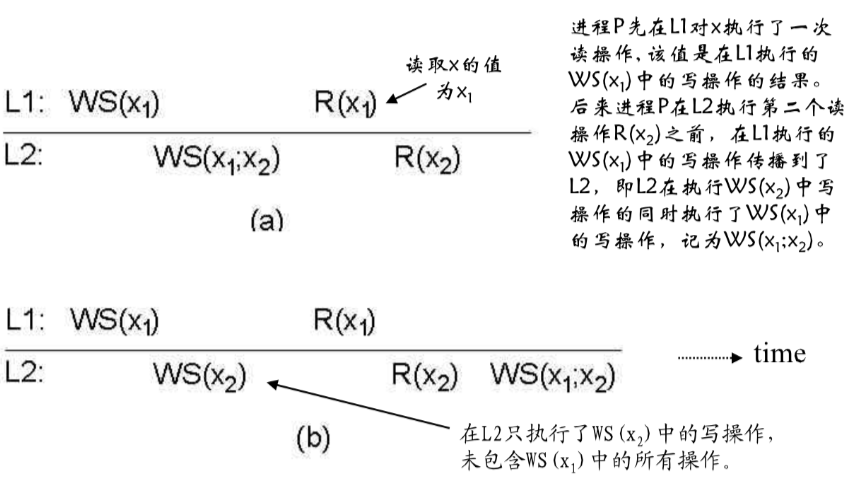
\includegraphics[width=0.4\textwidth,keepaspectratio]{pics/mono-read.png}

  \zhemph{单调写 monotonic-write consistency} 一个进程对数据项x执行的写操作必须在该进程对x执行任何后续写操作之前完成。两个写操作,前面那个写操作写完,后面那个写操作才写 每个写操作完全覆盖\emph{x}的当前值,但是没有必要更新副本。如果现在副本也要写,必须先完成之前的写操作。

  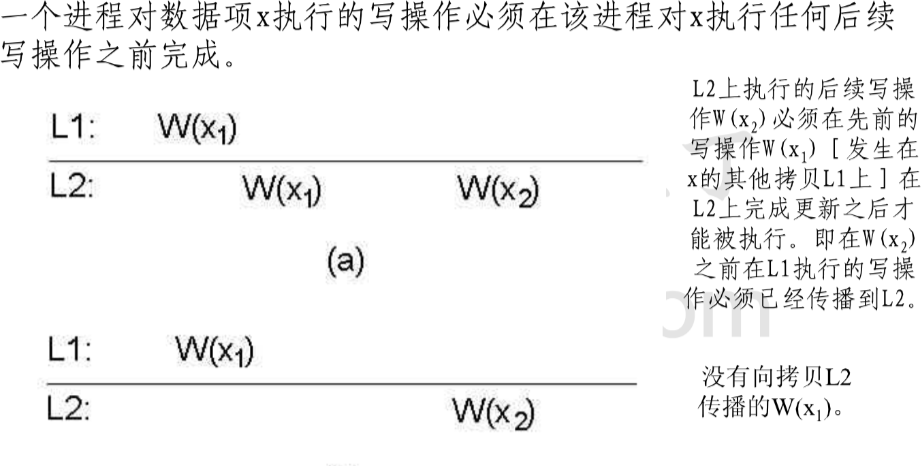
\includegraphics[width=0.4\textwidth,keepaspectratio]{pics/mono-write.png}

  \zhemph{读写一致性 read-your-writes consistency} 一个进程对数据项x执行一次写操作的结果总是会被该进程对x执行的后续读操作看见。
    
  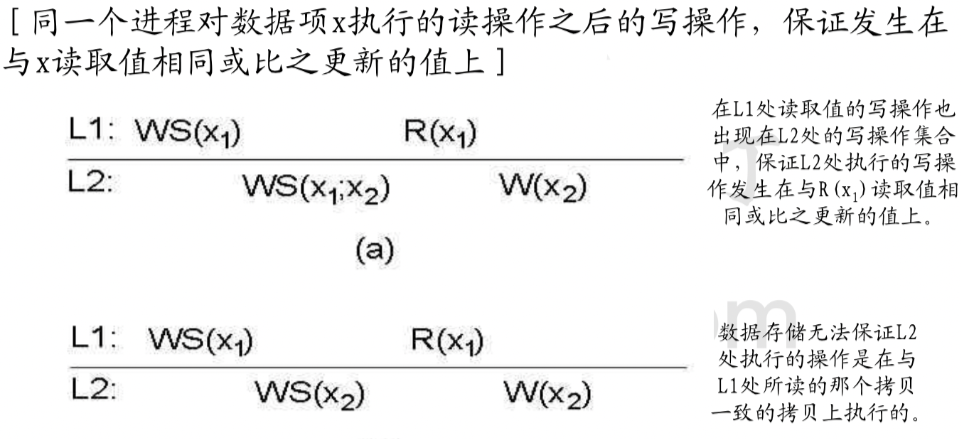
\includegraphics[width=0.4\textwidth,keepaspectratio]{pics/read-write.png}

  \zhemph{写读一致性 writes-follow-reads consistency} 同一个进程,对数据项x执行的读操作之后的写操作,保证发生在于x读值相同或比值更新的值上。 在x上所有接下来的写操作,应该是从上次读到的地方开始写,或者是比上次读到的结果还要新的地方开始写。

 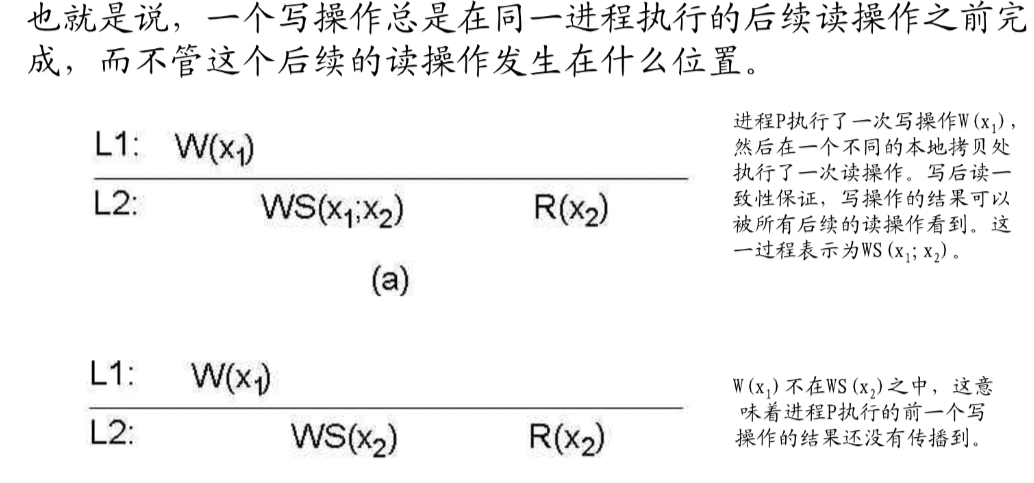
\includegraphics[width=0.4\textwidth,keepaspectratio]{pics/write-read.png}

\zhemph{内容复制与放置}
    
    从逻辑上,副本分为\textbf{永久副本、服务器启动的副本和客户启动的副本}。复制的顺序是永久副本 → 服务器启动的副本 → 客户启动的副本 → 客户。
    
    \textbf{永久副本}有两种:其一是将原始数据存储于处于同一数据中心的多台服务器中(分布式不一定要地理上分布很广,集群也是分布式的),做一个比较集中的负载均衡;其二是静态配置的镜像,地理上散布于互联网的各处。永久副本一般起到备份的作用。\textbf{服务器启动的副本}是应对压力动态、自动化创建的:如果某个地区的用户突然增多,就会自动在该地区创建(只读的)副本。这件事主要是 CDN 在做。\textbf{客户启动的副本}其实就是客户端缓存。
    
    第一个设计决策是传播什么信息。第一种可能是\textbf{传播通知},即通知这部分数据是无效的,不需要再复制了。在读写比很低、压倒性的写入密集型应用中,无效的中间状态很多,这种方法很有效。缓存系统也需要传递失效信息触发缓存更新,当然这种方法必然要和其他方法结合使用。第二种可能是\textbf{传播数据本身},传播数据、传播更新还是传播日志都算。第三种可能是\textbf{主动复制},即将更新操作发送给副本服务器。例如,将所有副本抽象为状态机,然后传播状态转移序列。实际上,有一种复制方案就是在加入限制后传播 SQL 语句。
    
    第二个设计决策是谁发起复制。第一种可能是\textbf{推式复制},即服务器主动分发数据,一般用于永久副本和服务器启动的副本。这种方式对源站并不透明,只对用户一侧单向透明,大型网站会考虑使用。例如,双十一之前,淘宝就在你的手机中预载了广告,这就是一种推式复制。第二种可能是\textbf{拉式复制},即客户请求 + 无数据/数据过期时才触发复制,一般用于高速缓存。这种方式可以做到完全的双向透明,是小型站点的首选。
    第三个设计决策是单播和多播,\textbf{拉式一般配合单播,推式一般配合多播。}  
  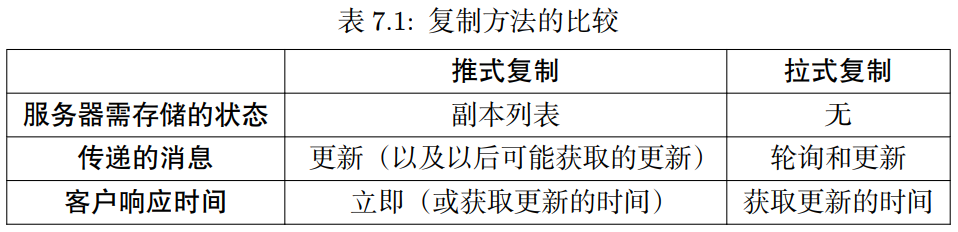
\includegraphics[width=0.45\textwidth,keepaspectratio]{pics/pull-push.png}

\zhemph{一致性协议}
  
  \zhemph{Primary-Based Protocols 基于主备份的协议}  远程写协议、本地写协议
  
  \zhemph{Replicated-Write Protocols 复制的写协议} 规定:一个服务器集群有N个机器,每个机器上都有这个文件。若要更新这个文件,客户必须先联系至少$\frac{N}{2}+1$个服务器,并得到他们同意后自行更新。一旦他们更新,该文件将被修改,这个新文件也将与一个新版本号关联,该版本号用于识别文件的版本,对于所有新更新的文件,他们的版本号是相同的。在读取的时候,有两种版本:
  
  a) 联系至少$\frac{N}{2}+1$个服务器,请求他们返回该文件关联的版本号。
  
  b) 根据$N_R$和$N_W$来计算,$N_W$越大,$N_R$就可以越小。
  
  1.一个客户要读取一个具有N个副本的文件,必须组织一个读团体(read quorum)该读团体是任意$N_R$个以上服务器的集合。
  2.要求改一个文件,客户必须组织一个至少有$N_W$个服务器的写团体。
  
  $N_R$和$N_W$满足以下条件:
  (1)$N_R$+$N_W$>N:\zhemph{防止读写操作冲突}
  (2)$N_W$>$\frac{N}{2}$:\zhemph{防止写写操作冲突}

  \section{容错 - Fault Tolerance} \zhemph{Fault tolerance容错} 构建一个组件,使其能够在出现故障时满足其规范 (即掩盖故障的存在)。\zhemph{可靠性dependable是一个术语,它包含了分布式系统中很多有用的需求:} 1.\zhemph{可用性:}被定义为系统的一个属性,他说明系统已准备好,马上可以使用 2.\zhemph{可靠性:}指系统可以无故障的持续运行。 3.\zhemph{安全性:}是指系统偶然出现故障的情况下能正确操作而不会造成任何灾难。 4.\zhemph{可维护性:}是指发生故障的系统被恢复难易程度\zhemph{Fault的类型} 1.\zhemph{短暂故障:}只发生一次,然后就消失了,即使重复操作也不会发生 2.\zhemph{间歇故障:}发生,消失不见,然后再次发生,如此反复进行。3.\zhemph{持久故障:}是那些知道故障组件被修复之前持续存在的故障\zhemph{Failure Models} \zhemph{1.Crash failures崩溃性故障}:服务器过早的停机,但是在停机之前工作正常。\zhemph{2.Omission failures:遗漏性故障}:服务器不能对请求进行响应,分为接受遗漏性故障和发送遗漏性故障。\zhemph{3.Timing failures定时故障:} 响应是正确的,但是在指定的时间范围之外,结果是正确的,但是时间不满足要求。\zhemph{4.Response failures响应故障:} 服务器响应不正确,分两种,数值故障,状态转换故障。\zhemph{5.Arbitrary (byzantine) failures随意性故障(也称为拜占庭故障):} 服务器可能产生任意输出并受到任意定时故障的影响,最严重的问题(没错也是Lamport提出来的)\zhemph{处理容错} 处理容错问题常常使用冗余来解决,例如海明码,物理冗余(多个硬件)。


  \zhemph{拜占庭将军问题} 为了保证下一步军事行动的一致性,将军们需要1.忠诚的将军最终的决定是一致的。(背叛者可以按照自己的意愿做决定)2.少数的背叛者不能导致忠诚的将军做出错误的决定。分布式系统中,没有服务器的存在,所以只能每个节点各自做决定。现在已知网络通讯是可靠的,但是存在不可靠的节点(叛徒)。需要找到一个算法,每个服务器都使用这个算法来做决策,有叛徒存在的情况下(因为有的节点会出错),至少需要多少个节点,可以做到:1.所有正常的结点,做出的决定是一致的;2.出错的节点不会影响到正常的节点做决定。
  
  \zhemph{投票 - Voting} 总结点数为n,其中有m个结点出错. 投票需要少数服从多数,所以当$n≥2m+1$时,能满足要求。
  
  \zhemph{口头消息 - Oral Message} A给B发送一则口头消息,B仅知道这个消息是A发来的,但是不知道这个消息是A产生的,还是A从别的那里转发来的。 \zhemph{前提条件} 1.消息会被正确地传送。 2.接受者知道此消息谁发的。3.如果有人不发消息,也是可以被检测到的。 当$n≥3m+1$时,能满足要求. 
  
  \zhemph{带签名的消息 - Sign Message} 在Oral Message的前提条件里再添加两个条件:1.忠诚的将军的签名不能被修改,对忠诚的将军的发出的消息的修改能够被检测到。 2.任何人都可以验证签名的真实性。当$n≥m+2$时,能满足要求。
  
  \zhemph{故障检测} \zhemph{核心思想} 通过超时机制来检测某个进程是否发生了故障 \zhemph{问题} 无法区分是由于网络不可靠还是由于进程出现了故障导致的超时。

  \zhemph{可靠通信} 远程过程调用(RPC)中的五种失败形式:1.客户不能定位服务器 2.客户到服务器的请求消息丢失 3.服务器在收到请求之后崩溃 4.从服务器到客户的响应消息丢失 5.客户在发送请求之后崩溃   \zhemph{解决方法} 1.\textbf{客户不能定位服务器}: 让错误抛出一个异常 2.\textbf{客户到服务器的请求消息丢失} 使操作系统或客户存根在发送请求时开启一个定时器,如果定时器超时了还没有收到应答,就重发消息。只需重新发送消息(并使用messageID唯一标识消息)  3.\textbf{服务器在收到请求之后崩溃} \textbf{对服务器的期望}:1.至少一次语义:在服务器重启之前(或者重新绑定到一个新的服务器之前)等待并再次尝试操作。2.最多一次语义:立即放弃并报告失败。 \textbf{客户可采取的4种策略}:1.不重发2.总是重发3.没有接收到第一次请求已经传送到服务器的确认时才重发4.只有接受到服务器发送的请求确认时才重发  
  
  4.\textbf{从服务器到客户的响应消息丢失}1.按幂等的方式组织所有的请求2.改进版:客户为每一个请求分配一个序列号,通过在服务器上跟踪从每个客户收到的最近序列号,服务器可以分辨原始的请求与重发的请求,并拒绝执行第二次发出的请求,但是服务器还是要向客户发送响应。
  
  5.\textbf{客户在发送请求之后崩溃(孤儿问题)}孤儿:如果客户向服务器发送请求,请求做一些事情,但是在服务器回复之前就崩溃了,这时虽然计算是活动的,但是没有双亲等待结果,这种不需要的计算称为孤儿计算。解决办法(4个)1.\textbf{孤儿消灭extermination} 在客户存根发送RPC消息之前进行进行日志记录来说明要做什么。在客户端重启之后,对日志进行检查然后明确的杀死孤儿。2.\textbf{再生reincarnation} 当客户端重启时,就向所有的机器广播一个消息说明一个新时期的开始,当这样的广播到达后,所有与那个客户有关的远程计算都被杀死。  3.\textbf{优雅再生gentle reincarnation} 当时期广播到达时,每台机器都进行检查来查看是否存在远程计算,如果有,就尝试定位他的拥有者,只有当不能找到拥有者的时候才杀死该孤儿。  4.\textbf{到期expiration} 每个RPC都被给定一个标准的时间量T来进行工作,如果到时不能结束,就必须显示的请求另外的时间量。(类似于租约)

  \emph{Paxos}
  
  Paxos 算法,它将分布式系统中的节点分为三类:\zhemph{提案节点(Proposer)}、\zhemph{决策节点(Acceptor)}和\zhemph{记录节点(Learner)}。Paxos 有三个阶段:
  
  \zhemph{(阶段1a)} 提案节点收到来自客户端的请求后,选择一个最新的提案编号$n$,向超过半数的决策节点广播Prepare消息,请求决策节点对提案编号进行投票。决策节点收到Prepare 消息后,如果提案编号$n$大于该节点已经批准的最大提案编号,则该节点批准提案编号$n$,并向提案节点发送批准消息;否则,该节点拒绝提案编号$n$,并向提案节点发送拒绝消息。
  
  \zhemph{(阶段1b)} 决策节点收到提案节点的提案编号$n$后,如果提案编号$n$大于该节点已经批准的最大提案编号,则返回Promise 消息。如果决策节点之前已经批准了某个提案,那么Promise 消息还应将前一次提案的编号和对应的值一起发送给提案节点,否则回复null. 发送Promise 信息后,决策节点承诺:不再接受提案编号小于等于当前请求的Prepare 请求;不再接受提案编号小于当前请求的Propose 请求。
  
  \zhemph{(阶段2a)} 提案节点收到超过半数的决策节点的Promise 消息后,向多数派的决策节点发起Accept 请求,带上提案编号和提案值。关于提案的值的选择,如果之前决策节点的Promise 消息有返回已接受的值,那么使用提案编号最大的已接受值作为提案值;如果没有返回任何已接受值,那么提案节点可以自由决定提案值。
  
  \zhemph{(阶段2b)} 决策节点收到Accept 请求后,若没有承诺过提案编号比$n$更大的提案,则决策节点接受该提案,更新承诺的提案编号,保存已接受的提案,并向提案节点发送Accepted 消息;否则,决策节点拒绝该提案,向提案节点发送Rejected 消息。
  
  \zhemph{(阶段3)} 提案节点收到超过半数的决策节点的Accepted 消息后,将提案值作为决策结果提交给所有记录节点。否则,延迟一段时间并重启整个过程。
  
  Paxos 能在部分同步系统和崩溃故障下达成共识,只需$N≥2f+1$,但不能容忍拜占庭故障。PBFT 算法(Practical Byzantine Fault Tolerance)是拜占庭容错算法的改进,使用了加密算法,能在$N≥3f+1$的条件下容忍拜占庭故障,且通信复杂度为$O(n^2)$。

  \section{云计算} \zhemph{网格计算} 1.在动态变化、由多个机构组成的虚拟组织中协调资源共享和求解问题 2.实现跨组织跨平台异构资源的共享 \zhemph{云计算} 1.一种\zhemph{商业}计算模型。2.将计算任务分布在大量计算机构成的资源池上,使各种应用系统(用户)能够根据需要获取计算力、存储空间和信息服务。

  \zhemph{文件系统的存储内容}
  
  主要内容:用户的实际数据
  
  元数据:驱动器元数据与文件元数据
  
  \zhemph{Google云计算平台技术架构} 1.文件存储 Google Distributed File System,GFS 2.并行数据处理MapReduce 3.分布式锁 Chubby 4.结构化数据表 BigTable
  
  \zhemph{GFS的假设与目标} 1.硬件出错是正常而非异常 (a.系统应当由大量廉价、易损的硬件组成 b.必须保持文件系统整体的可靠性) 2. 主要负载是流数据读写 (a.主要用于程序处理批量数据,而非与用户的交互或随机读写 b.数据写主要是``追加写'',``插入写''非常少) 3. 需要存储大尺寸的文件 (存储的文件尺寸可能是GB或TB量级,而且应当能支持存储成千上万的大尺寸文件) 
  
  \zhemph{GFS的设计思路} 1.将文件划分为若干块(Chunk)存储 每个块固定大小(64M) 2.通过冗余来提高可靠性 每个数据块至少在3个数据块服务器上冗余 3.通过单个master来协调数据访问、元数据存储 结构简单,容易保持元数据一致性 4.无缓存

  \zhemph{GFS架构的特点} .采用中心服务器模式 1.可以方便地增加Chunk Server 2.Master掌握系统内所有Chunk Server的情况,方便进行负载均衡 3.不存在元数据的一致性问题 4.不缓存数据 5.在用户态下实现 6.提供专用的访问接口 
  
  \zhemph{GFS的容错方法} 1.\zhemph{Chunk Server容错机制} 每个Chunk有多个存储副本(通常是3个),分别存储于不通的服务器上; 每个Chunk又划分为若干Block(64KB),每个Block对应一个32bit的校验码,保证数据正确(若某个Block错误,则转移至其他Chunk副本)2.\zhemph{Master容错(影子节点热备)}三类元数据:命名空间(目录结构)、Chunk与文件名的映射(写日志提供容错)以及Chunk副本的位置信息; 前两类通过日志提供容错,Chunk副本信息存储于Chunk Server,Master出现故障时可恢复

  \zhemph{MapReduce} 实现了Map和Reduce两个功能 1.Map把一个函数应用于集合中的所有成员,然后返回一个基于这个处理的结果集2.Reduce对结果集进行分类和归纳3.Map()和 Reduce() 两个函数可能会并行运行,即使不是在同一的系统的同一时刻
  
  \zhemph{为什么需要MapReduce?}1.海量数据在单机上处理因为硬件资源限制,无法胜任 2.而一旦将单机版程序扩展到集群来分布式运行,将极大增加程序的复杂度和开发难度3.引入 MapReduce 框架后,开发人员可以将绝大部分工作集中在业务逻辑的开发上,而将分布式计算中的复杂性交由框架来处理。
  
  \zhemph{Google MapReduce执行流程 1.}一个MapReduce程序启动的时候,最先启动的是 MRAppMaster, MRAppMaster 启动后根据本次 job 的描述信息,计算出需要的 maptask 实例数量,然后向集群申请机器启动相应数量的 maptask 进程2.maptask 进程启动之后,根据给定的数据切片(哪个文件的哪个偏移量范围)范围进行数据处理3.MRAppMaster 监控到所有 maptask 进程任务完成之后(真实情况是,某些 maptask 进 程处理完成后,就会开始启动 reducetask 去已完成的 maptask 处 fetch 数据),会根据客户指 定的参数启动相应数量的 reducetask 进程,并告知 reducetask 进程要处理的数据范围(数据分区)4.Reducetask 进程启动之后,根据 MRAppMaster 告知的待处理数据所在位置,从若干台 maptask 运行所在机器上获取到若干个 maptask 输出结果文件,并在本地进行重新归并排序, 然后按照相同 key 的 KV 为一个组,调用客户定义的 reduce()方法进行逻辑运算,并收集运算输出的结果 KV,然后调用客户指定的 outputformat 将结果数据输出到外部存储

  \zhemph{MapReduce的容错Worker故障} 1.Master 周期性的ping每个worker。如果master在一个确定的时间段内没有收到worker返回的信息,那么它将把这个worker标记成失效 2.重新执行该节点上已经执行或尚未执行的Map任务 3.重新执行该节点上未完成的Reduce任务,已完成的不再执行  \zhemph{Master故障} 1.定期\zhemph{写入检查点数据} 2.从\zhemph{检查点}恢复

  \zhemph{Chubby} \zhemph{是Google设计的提供粗粒度锁服务的一个文件系统,主要用于解决分布式一致性问题。} Chubby系统本质上就是一个分布式的、存储大量小文件的文件系统:
    1. Chubby中的锁就是文件
    2. 创建文件就是进行“加锁”操作,创建文件成功的那个server其实就是抢占到了“锁”
    3. 用户通过打开、关闭和存取文件,获取共享锁或者独占锁;并且通过通信机制,向用户发送更新信息
    
  
  \zhemph{BigTable} \zhemph{BigTable概述} 基于GFS和Chubby的分布式存储系统 1.对数据进行\zhemph{结构化}存储和管理 2.与GFS的联系,存到底层都是GFS \zhemph{BigTable和数据库的Table可完全不一样:} 1.数据库的table有外键关联,有实体之间的关系;2.BigTable没有关系这一说,是nosql,不支持关系操作。(而且云存储一般都不支持)

  \zhemph{BigTable数据模型} \zhemph{行} 1.每行数据有一个可排序的关键字和任意列项,即key 2.字符串、整数、二进制串甚至可串行化的结构都可以作为行键 3.表按照行键的``逐字节排序''顺序对行进行有序化处理 4.表内数据非常`稀疏',不同的行的列的数完全目可以大不相同 4.URL是较为常见的行键,存储时需要倒排 \zhemph{列} 1.特定含义的数据的集合,如图片、链接等 2.\zhemph{可将多个列归并为一组,称为族(family)} 3.采用 族:限定词 的语法规则进行定义 \zhemph{时间戳} 保存不同时期的数据,如``网页快照'' 
  
  \emph{A big table} 1.表中的列可以不受限制地增长 2.表中的数据几乎可以无限地增加 \zhemph{无数据校验} 1.每行都可存储任意数目的列 \zhemph{BigTable不对列的最少数目进行约束} 2.任意类型的数据均可存储 \zhemph{BigTable将所有数据均看作为字符串} 数据的有效性校验由构建于其上的应用系统完成 \zhemph{一致性} 针对同一行的多个操作可以分组合并 \zhemph{不支持对多行进行修改的操作符}

\end{multicols}


\end{document}